\chapter{Knowledge Acquisition}\label{ch:Knowledge Acquisition}

% Finished analysis of the applicable concepts and a collection of the concepts to be used in the ontology describing multiagent systems, i.e. the refined first glossary with potentially relevant terms and their meaning.

\blockquote[{{\cite[p. 37]{fernandez-lopez1997METHONTOLOGYOntologicalArt}}}]{It is important to bear in mind that knowledge acquisition is an independent activity in the ontology development process. However, it is coincident with other activities. \textelp{} Most of the acquisition is done simultaneously with the requirements specification phase and decreases as the ontology development process moves forward.}

The authors of METHONTOLOGY describe knowledge acquisition as a process that lasts throughout the ontology engineering process, yet it is not always of the same intensity. Early engineering process steps are richer in knowledge acquisition, classification and modelling. The main goal of this step is to identify sources of knowledge used as input for the remaining steps and to extract and acquire the knowledge necessary for successfully engineering the planned ontology.

This ontology's primary source of concepts, information, and knowledge is the MAMbO5 ontology presented in more detail in \cite{okresaduric2019MAMbO5NewOntology}. MAMbO5 results from an earlier collaboration instance of the sending and host institution, particularly this mobility's young researcher and the hosting research institute. The main goal of that ontology is to provide concepts related to modelling a multiagent system as an \ac{IVE}, boosted with concepts used in describing the organisational features of a system of agents. An \ac{IVE} in this context is a virtual system that can be seen as a model of a real system comprising agents, artefacts, and many other concepts related to the two. The agent and the artefact concepts are expected to be specialised for specific application areas when modelling a domain-specific scenario.

The purpose of MAGO-A ontology is to enable modelling a \ac{MAS} in a way that is translatable into implementation, specifically in the SPADE-based implementation foundation of the modelled system. To do so, some concepts of the MAMbO5 ontology have to be modified and some added, while the rest of the concepts can be left in the ontology for expressiveness and comprehensiveness. For knowledge acquisition in this part of the planned research and enhancing collaboration with the host institute, guided meetings have been performed, followed by structured brainstorming sessions and research plans, with the research team of Dr Carrascosa. Since the goal of this part of the planned research is aligned with a part of the research performed by Dr Carrascosa and his team, the rest of the planned research is conducted in cooperation with them.

Building on the MAMbO5 ontology, the MAGO-A ontology is planned to comply with the digital twin concept and the idea of containing concepts applicable to instantiating a \ac{MAS} based on the model expressed using the developed ontology. Therefore, it must include some concepts related to the implementation domain, e.g., describing agents' internal variables or the knowledge models used. The following is an overview of the selection of the more interesting concepts, followed by a selection of the concepts that have to be added. Both the described tables include the concepts identified as such and are not necessarily exhaustive.


\section{Glossary}

\newthought{Agent}
    \marginnote{Overview of the select concepts contained in MAMbO5 ontology}%
\blockquote[{{\cite[p. 54]{russell2022ArtificialIntelligenceModern}}}]{An agent is anything that can be viewed as perceiving its environment through sensors and acting upon that environment through actuators.} 

\newthought{Organisational unit} An organisational unit is an \mintedInline{Agent} subclass that is a part of an organisation. Usually, a \ac{MAS} can be considered an organisation comprising multiple agents. Strictly speaking, it would have to feature and use some other concepts related to defining, e.g. organisational structure. An organisational unit can be a part of another organisational unit and consist of organisational units. This feature, similar to the concept of holons and holarchy, allows for modelling organisations on different levels of abstraction or hierarchy. Each \mintedInline{OrganisationalUnit} instance is expected, at any given point in time, to be able to enact one of a set of \mintedInline{Role} individuals at its disposal. 

\newthought{Behaviour} The concept of agent behaviour is described in the \mintedInline{ooooaflsmas} ontology as \blockquote{\textelp{} some kind of activity performed by some agent. It has to be acceptable by a normative system the agent belongs to.} In terms of SPADE implementation, behaviour is the most basic way of implementing the operations of an agent. Each agent can have multiple behaviours. Types of behaviours offered by default by SPADE can already be found in the \mintedInline{ooooaflsmas} ontology,
\lookAt{\cref{fig:behaviour subclasses in ooooaflsmas}}%
i.e., one-shot, periodic, and finite state behaviour that acts according to the principles of finite automata. Each \mintedInline{Behaviour} individual is expected to provide its \mintedInline{Agent} individual with the ability to achieve a certain objective. Some innate \mintedInline{Behaviour} individuals will be available to specific \mintedInline{Agent} subclasses by default.

\begin{figure}
    \centering
    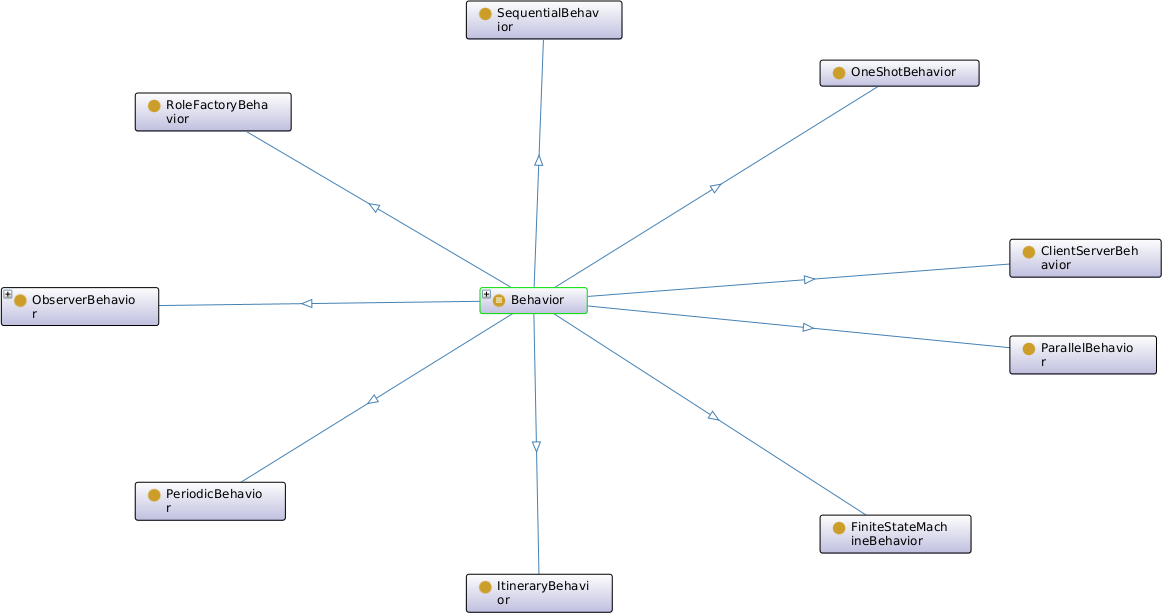
\includegraphics[width=0.84\linewidth]{Deliverables/Phase 1.1/Figures/Behaviours in ooooaflsmas.png}
    \caption{Subclasses of the \mintedInline{Behavior} concept in \mintedInline{ooooaflsmas}}
    \label{fig:behaviour subclasses in ooooaflsmas}
\end{figure}

\newthought{Role} The concept of a role is described within the \mintedInline{ooooaflsmas} ontology as a \blockquote{prescribed or expected behavior associated with a particular position or status in a group or organization}. This concept is in the mentioned ontology designated as a direct subclass of the concept \mintedInline{Norm}, derived from the domain of organisational modelling and describing organisation systems. The \mintedInline{Norm} concept is defined therein as \blockquote{(socially) accepted behavior in a defined group and \textins{they} represent a blueprint for behaving in said group.} Based on the stated, the concept of \mintedInline{Role} is interesting because it enables defining a set of features that will be put at the agent's disposal playing the chosen role. In other words, roles can be used as a way of combining different features that can be enacted by an agent. The \mintedInline{Role} concept was modelled in \cite{okresaduric2019OrganizationalModelingLargeScale} as a concept which was related to (possibly) several instances of concepts describing behaviours and objectives, meaning that specific roles allow agents who enact them to attain a specific set of behaviours
\lookAt{\cref{fig:roles achieve objectives and enable knowledge}}%
that enables and empowers them to achieve specific objectives, thus solving specific tasks. Different objectives demand the enactment of various roles from the pool of roles available (defined) in the system. 

\begin{figure}
    \centering
    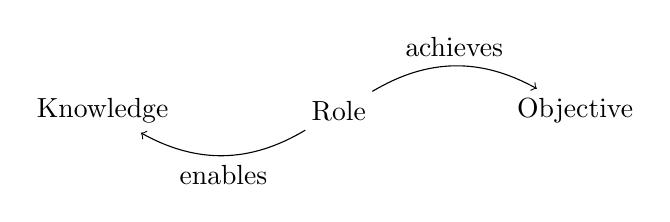
\begin{tikzpicture}
  % Nodes
  \node (K) at (-3,0) {Knowledge};
  \node (R) at (0,0) {Role};
  \node (O) at (3,0) {Objective};

  % Connections
  \draw[->] (R) to[bend left] node[midway, below] {enables} (K);
  \draw[->] (R) to[bend left] node[midway, above] {achieves} (O);
\end{tikzpicture}

    \caption{A \mintedInline{Role} individual can achieve some \mintedInline{Objective} individuals and can provide access to some \mintedInline{Knowledge} individuals}
    \label{fig:roles achieve objectives and enable knowledge}
\end{figure}

\newthought{Artefact} An artefact is used in the \mintedInline{JaCalIVE} ontology as a comprehensive concept encompassing all interactive and non-interactive objects that are not suitable to be implemented as agents, but should be present in the modelled system nonetheless. \mintedInline{MAMbO5} ontology recognises specific versions of artefacts as an \mintedInline{IVE_Artifact}, which is located within the \ac{IVE}, and its even more specific version \mintedInline{Physical_Artifact}, which can be physically represented or is expected to be physically represented, and a complementary specification given as a \mintedInline{KnowledgeArtifact} that is an artefact that is abstract and describes various rules that can be found within the modelled system. Its initial authors describe the latter concept as encompassing \enquote{a wide range of explicit knowledge,} including, but not limited to, knowledge models, such as machine learning models or neural networks. The \mintedInline{Norm} concept and its subclass \mintedInline{Role} are subclasses of the \mintedInline{KnowledgeArtifact} concept,
\lookAt{\cref{fig:Hierarchy artefact KNartefact norm role}}%
as defined in \mintedInline{ooooaflsmas}.

\begin{figure}
    \centering
    
\includegraphics[width=0.84\linewidth]{Deliverables/Phase 1.1/Figures/Hierarchy artefact KNartefact norm role.png}
    \caption{Class hierarchy on subclasses of the \mintedInline{Artifact} concept in \mintedInline{ooooaflsmas} ontology}
    \label{fig:Hierarchy artefact KNartefact norm role}
\end{figure}

\newthought{Stage} By definition, an \mintedInline{Agent} is located in an environment. Such an environment can comprise multiple agents and other entities, such as instances of the \mintedInline{Artefact} concept. During one of the brainstorming sessions on the topic of this research with the colleagues of the host institution (\acf{VRAIN} at the \ac{UPV}), a more specific environmental concept was discussed. Since the system described by this ontology is planned to be able to implement several more specific environments of the same domain, it is deemed useful to define a concept describing a smaller-scale environment. This is where the \mintedInline{Stage} concept comes in. In the context of this research, a stage should represent a smaller-scale environment, a specialised version of the general environment, that is related to the general domain of the modelled system.
Furthermore, a \mintedInline{Stage} individual groups related agents and artefacts together. It is possible to think of an individual of the \mintedInline{Stage} concept as a room or stage where a specific set of activities or processes is conducted. A single stage is envisioned as comprising some \mintedInline{Agent} individuals.
